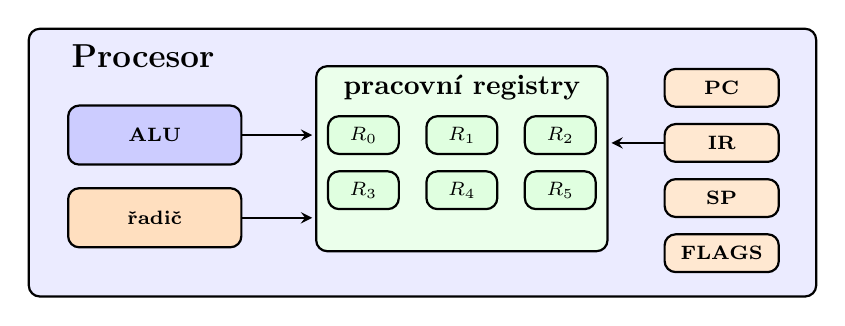
\begin{tikzpicture}[
    x=1cm, y=1cm,
    >=stealth,
    every node/.style={font=\scriptsize},
    cpu/.style={
        draw,
        thick,
        rounded corners,
        fill=blue!8,
        align=center
    },
    unit/.style={
        draw,
        thick,
        rounded corners,
        align=center,
        fill=white,
        minimum height=0.55cm
    },
    reg/.style={
        draw,
        thick,
        rounded corners,
        align=center,
        fill=green!12,
        minimum width=0.9cm,
        minimum height=0.48cm
    },
    special/.style={
        draw,
        thick,
        rounded corners,
        align=center,
        fill=orange!18,
        minimum width=1.45cm,
        minimum height=0.48cm
    },
    arr/.style={->, thick}
]

    % CPU outer box
    \node[
        cpu,
        minimum width=10.0cm,
        minimum height=3.4cm
    ] (cpu) at (0.25,0) {};

    \node[font=\large\bfseries] at (-3.3,1.35) {Procesor};

    % ALU and control
    \node[
        unit,
        fill=blue!20,
        minimum width=2.2cm,
        minimum height=0.75cm
    ] (alu) at (-3.15,0.35) {\textbf{ALU}};

    \node[
        unit,
        fill=orange!25,
        minimum width=2.2cm,
        minimum height=0.75cm
    ] (ctrl) at (-3.15,-0.70) {\textbf{řadič}};

    % General registers block title
    \node[
        unit,
        fill=green!8,
        minimum width=3.7cm,
        minimum height=2.35cm
    ] (regfile) at (0.75,0.05) {};

    \node[font=\bfseries] at (0.75,0.95) {pracovní registry};

    % Registers grid
    \node[reg] (r0) at (-0.50,0.35) {$R_0$};
    \node[reg] (r1) at (0.75,0.35) {$R_1$};
    \node[reg] (r2) at (2.00,0.35) {$R_2$};

    \node[reg] (r3) at (-0.50,-0.35) {$R_3$};
    \node[reg] (r4) at (0.75,-0.35) {$R_4$};
    \node[reg] (r5) at (2.00,-0.35) {$R_5$};

    % Special registers
    \node[special] (pc) at (4.05,0.95) {\textbf{PC}};
    \node[special] (ir) at (4.05,0.25) {\textbf{IR}};
    \node[special] (sp) at (4.05,-0.45) {\textbf{SP}};
    \node[special] (flags) at (4.05,-1.15) {\textbf{FLAGS}};

    % Arrows
    \draw[arr] (alu.east) -- (-1.15,0.35);

    \draw[arr] (ctrl.east) -- (-1.15,-0.70);
    \draw[arr] (ir.west) -- (2.65,0.25);

\end{tikzpicture}
